\chapter{Appendix to Chapter 5}
\label{chap:appendix_ch5}

\section{Simulation Details for Results in Section \ref{subsec:tparam_motivation}}
\label{sec:tparam_motiv_details}

\subsection{Simulation setup}
\label{subsec:tparam_motiv_setup}

We simulated an outbreak with SIRS dynamics in a population of $ N= 100,000$ individuals, ten of whom were initially infected, spanning two wave of the outbreak over thirty weeks. The mean infectious period duration was one week, and the mean duration of immunity was four weeks. The basic reproduction numbers of the outbreak, and hence the per--contact infectivity rates, varied sinusoidally with additive noise, over the course of the outbreak:
\begin{equation}
\label{eqn:sinfoi_true_R0t}
R0(t) = \beta(t) N / \mu = 2 + 0.35(\sin(t / 3.5) + 0.1Z_t),
\end{equation} 
where $ Z_t \sim N(0,1)$. The per--contact infection rates were then obtained as $ \beta(t) = R0(t) \mu / N $ The observed incidence was a negative binomial sample of the true incidence with mean case detection rate $ \rho $ and overdispersion parameter $ \phi $: 
\begin{equation}
Y_\ell \sim \mr{Neg.Binom.}\left (\mu  = \rho(N_{SI}(t_\ell) - N_{SI}(t_{\ell-1})), \sigma^2 = \mu(1 + \mu /\phi) \right ).
\end{equation}

We fit two models, one where the force of infection was constant over the course of the outbreak and another where the rates of infectious contact were time varying, with log--differences in the basic reproduction numbers penalized using a first order Gaussian Markov random field (GMRF) shrinkage prior where the standard deviation of the log--differences is given by $ \sigma_{RW1} $ (analogous to the models in Section \ref{sec:flu_tparam_models}). We employed non--centered parameterizations for both the LNA and the GMRF. The models were fit under informative priors, summarized in Table \ref{tab:tparam_sim_priors}. We ran five MCMC chains per model for 100,000 iterations per chain, alternating between five elliptical slice sampling (EllipSS) updates and one multivariate normal slice sampling (MVNSS) updates per MCMC iteration. The estimation scale on which the MCMC explored the parameter space was given by $\lbrace \log(R0(t_0)), \log(1/mu), \logit(\rho), 1/\sqrt(\phi) \rbrace$. The MVNSS proposal covariance matrix was adapted throughout the first 50,000 iterations, samples from which were subsequently discarded, using the gain factor sequence: the gain factor sequence, $\gamma_n = 0.5(1 + 0.01n)^{-0.99}$. The contribution of isotropic Gaussian noise to the MVNSS proposal was initialized at 0.001 and reduced throughout the adaptation phase according to the sequence $ \iota_n = 0.001(1 + 0.01n)^{-0.99} $. Convergence was assessed visually by inspection of traceplots of posterior samples, and via potential scale reduction factors (PSRFs) \cite{brooks1998general} computed via the \texttt{coda} R package \cite{codapackage}.

\begin{table}[htbp]
	\caption[Parameters and priors for models fit two SIRS models to data from a simulated outbreak with sinusoidal FOI.]{Parameters and priors used in fitting two SIRS models, one with constant FOI and another with time--varying FOI, to data from an outbreak with SIRS dynamics where the per--contact infection rate varied sinusoidally over time.}
	\label{tab:tparam_sim_priors}
	\scriptsize\centering
	\begin{tabular}{clllr}
		\hline
		\textbf{Parameter} & \textbf{Interpretation} & \textbf{Truth} & \textbf{Prior} & \textbf{Median (95\% Interval)} \\ \hline
		$ R0-1 $ & Basic reproduction \#-1 & (\ref{eqn:sinfoi_true_R0t}) & LogNormal(0, 0.5) & $ \implies R0(t_0) = $ 2.00 (1.14, 8.10) \\ 
		$ 1/\mu $ & Mean infectious period & 1&  LogNormal(0.05, 0.5)& 1.05 (0.39, 2.80) \\
		$ \rho/(1-\rho)  $ & Odds of case detection  &0.25&  LogNormal(-0.847, 0.5) & $ \implies \rho =$ 0.3 (0.14, 0.53) \\
		$ 1/\sqrt{\phi} $ & Neg.Binom. overdispersion & 50 & Exponential(5)& $ \implies \phi = 52 (1.84, 39000) $.  \\
		\hline
	\end{tabular}
\end{table}

\subsection{Additional results}
\label{subsec:sinfoi_supp_res}

\begin{figure}[htpb]
	\centering
	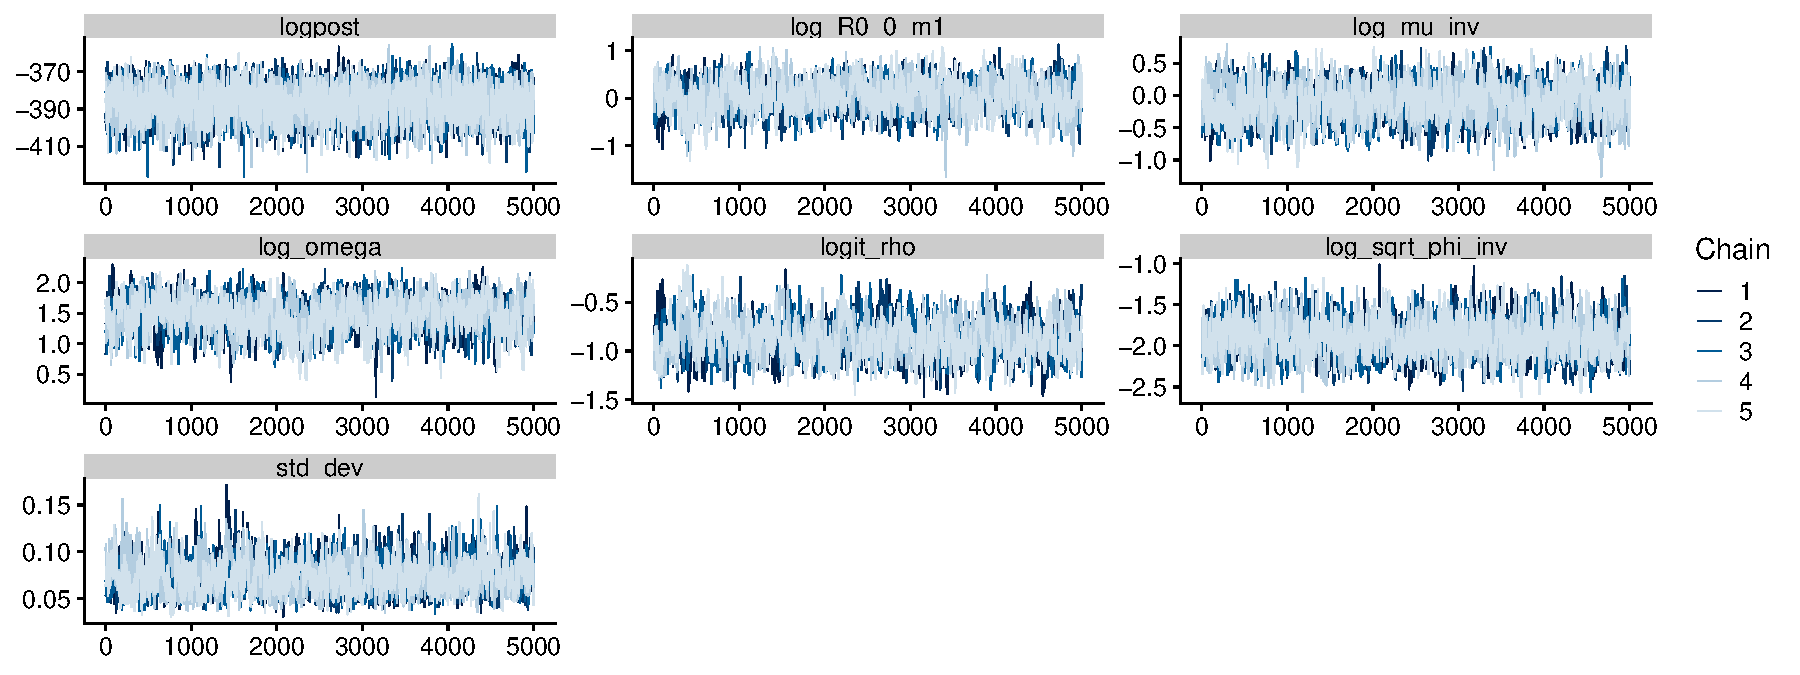
\includegraphics[width=\linewidth]{figures/sinfoi_rw1_traces}
	\caption{Posterior traceplots for SIRS model parameters with time--varying force of infection.}
	\label{fig:sinfoirw1traces}
\end{figure}

\begin{figure}[htpb]
	\centering
	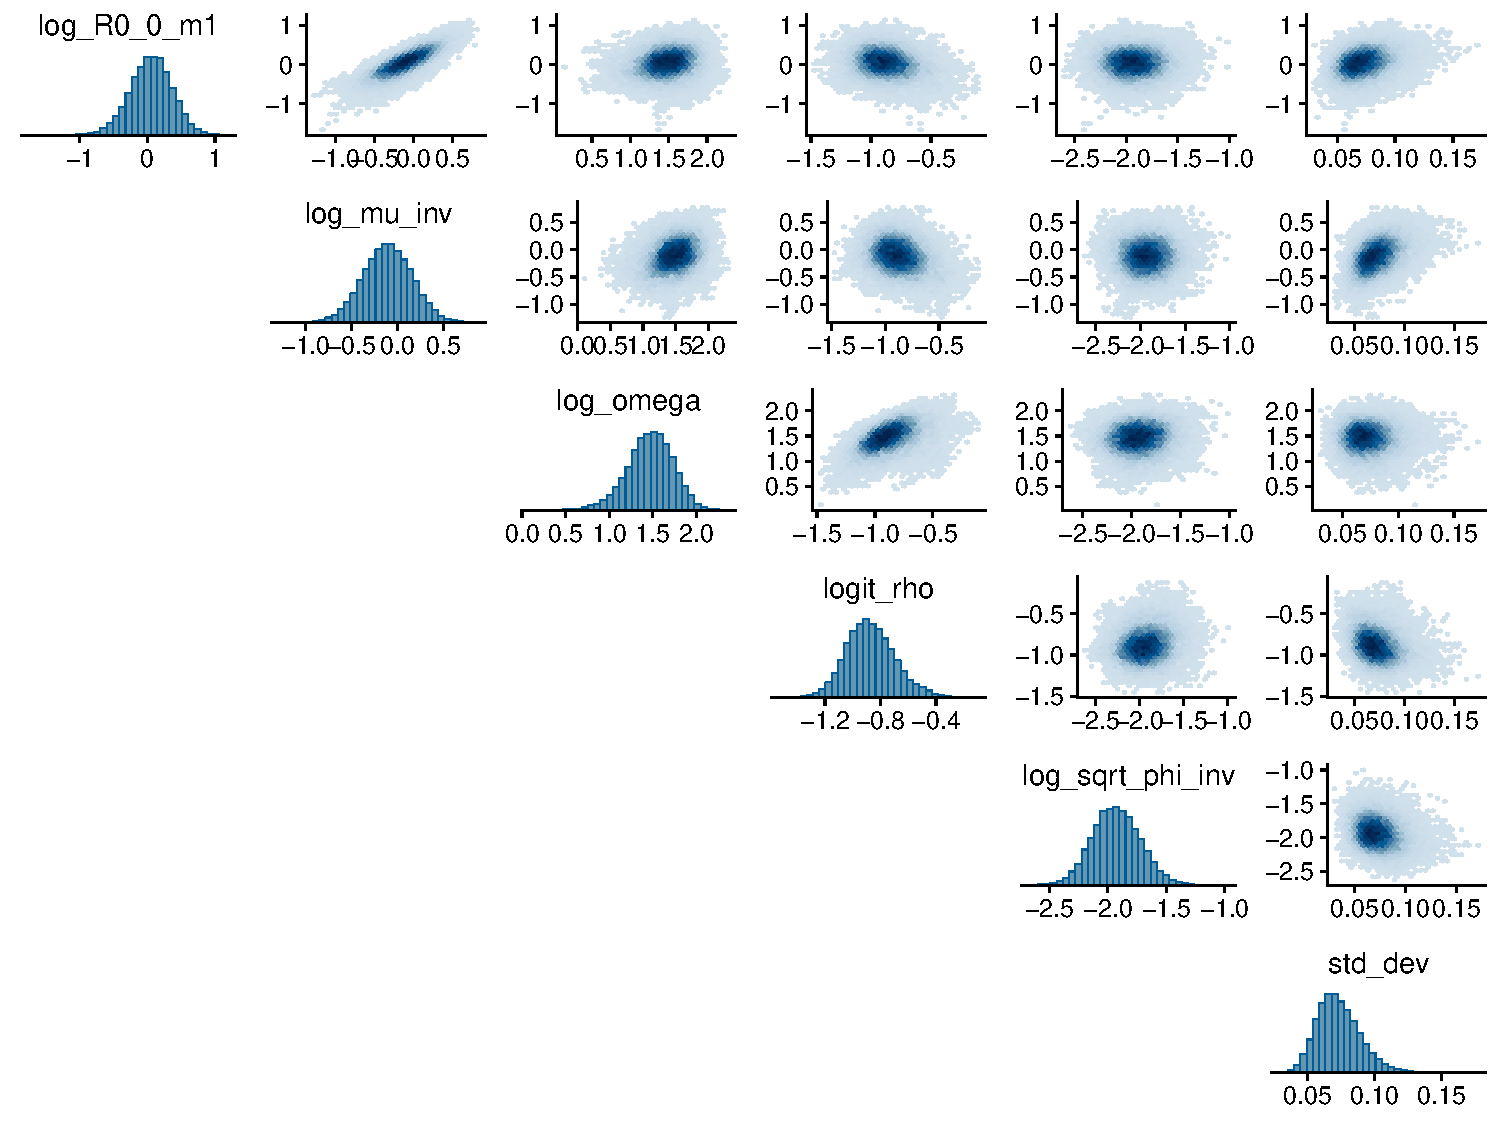
\includegraphics[width=\linewidth]{figures/sinfoi_rw1_pairs}
	\caption{Posterior histograms and pairwise hexplots for SIRS model parameters with time--varying force of infection.}
	\label{fig:sinfoirw1pairs}
\end{figure}

\begin{figure}[htpb]
	\centering
	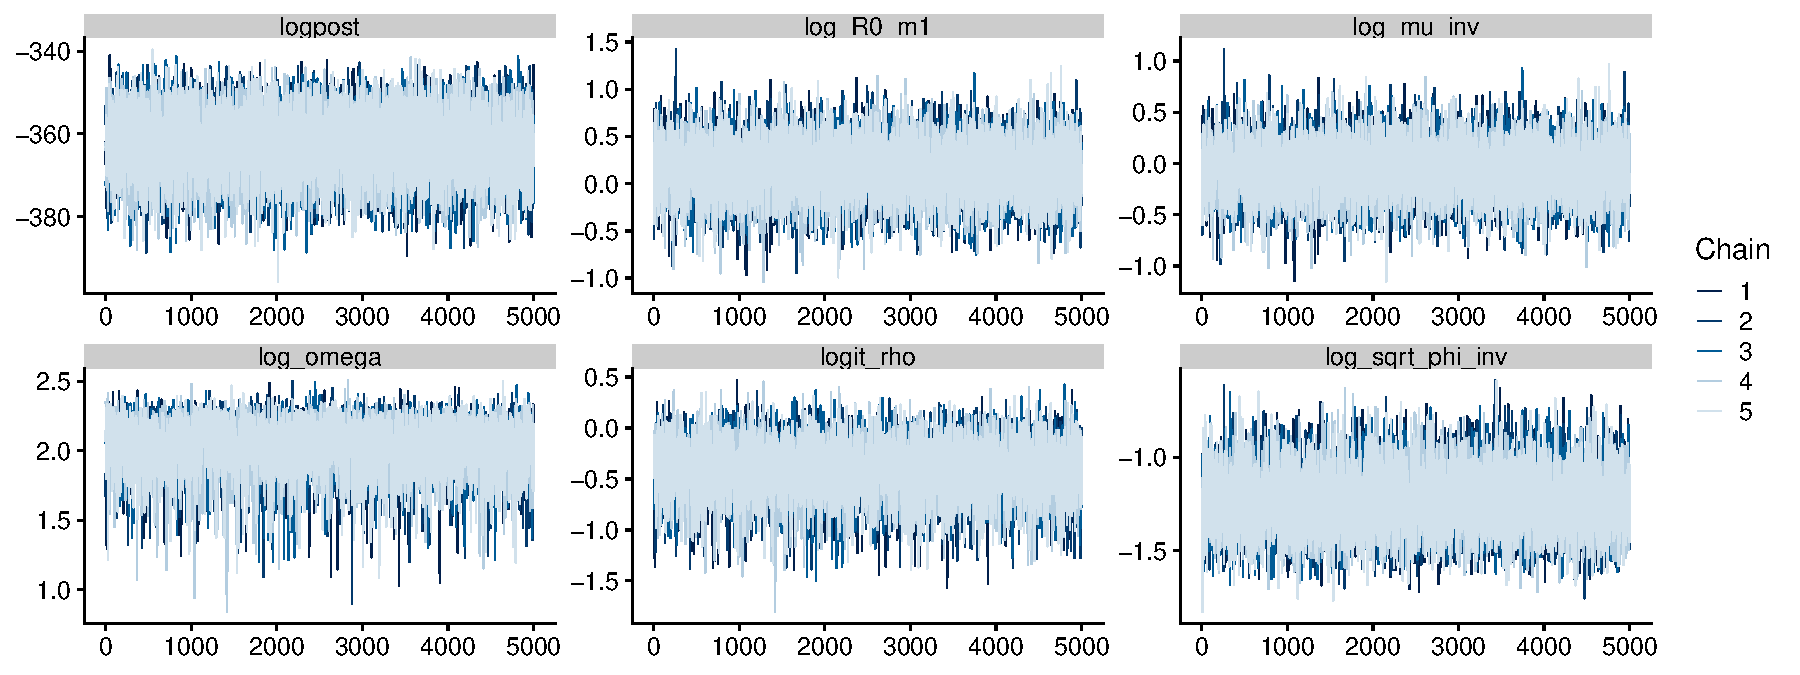
\includegraphics[width=\linewidth]{figures/sinfoi_const_traces}
	\caption{Posterior traceplots for SIRS model parameters with time--homogeneous force of infection.}
	\label{fig:sinfoiconsttraces}
\end{figure}

\begin{figure}[htpb]
	\centering
	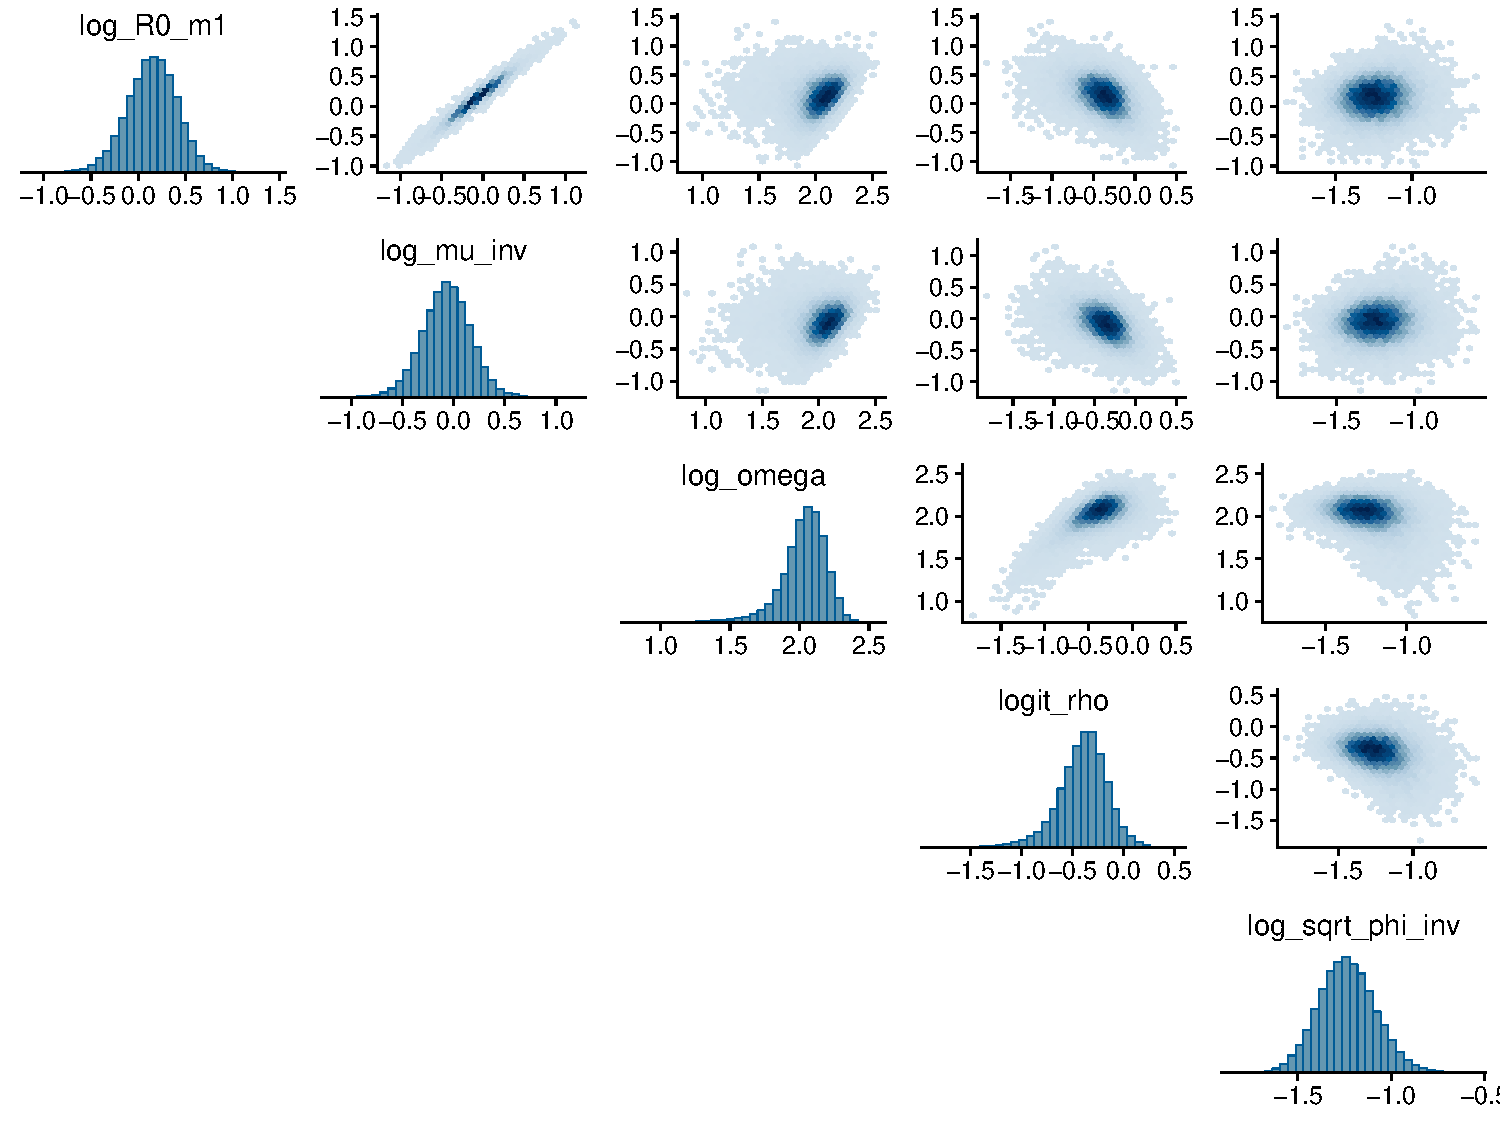
\includegraphics[width=\linewidth]{figures/sinfoi_const_pairs}
	\caption{Posterior histograms and pairwise hexplots for SIRS model parameters with time--homogeneous force of infection.}
	\label{fig:sinfoiconstpairs}
\end{figure}

\begin{figure}[htpb]
	\centering
	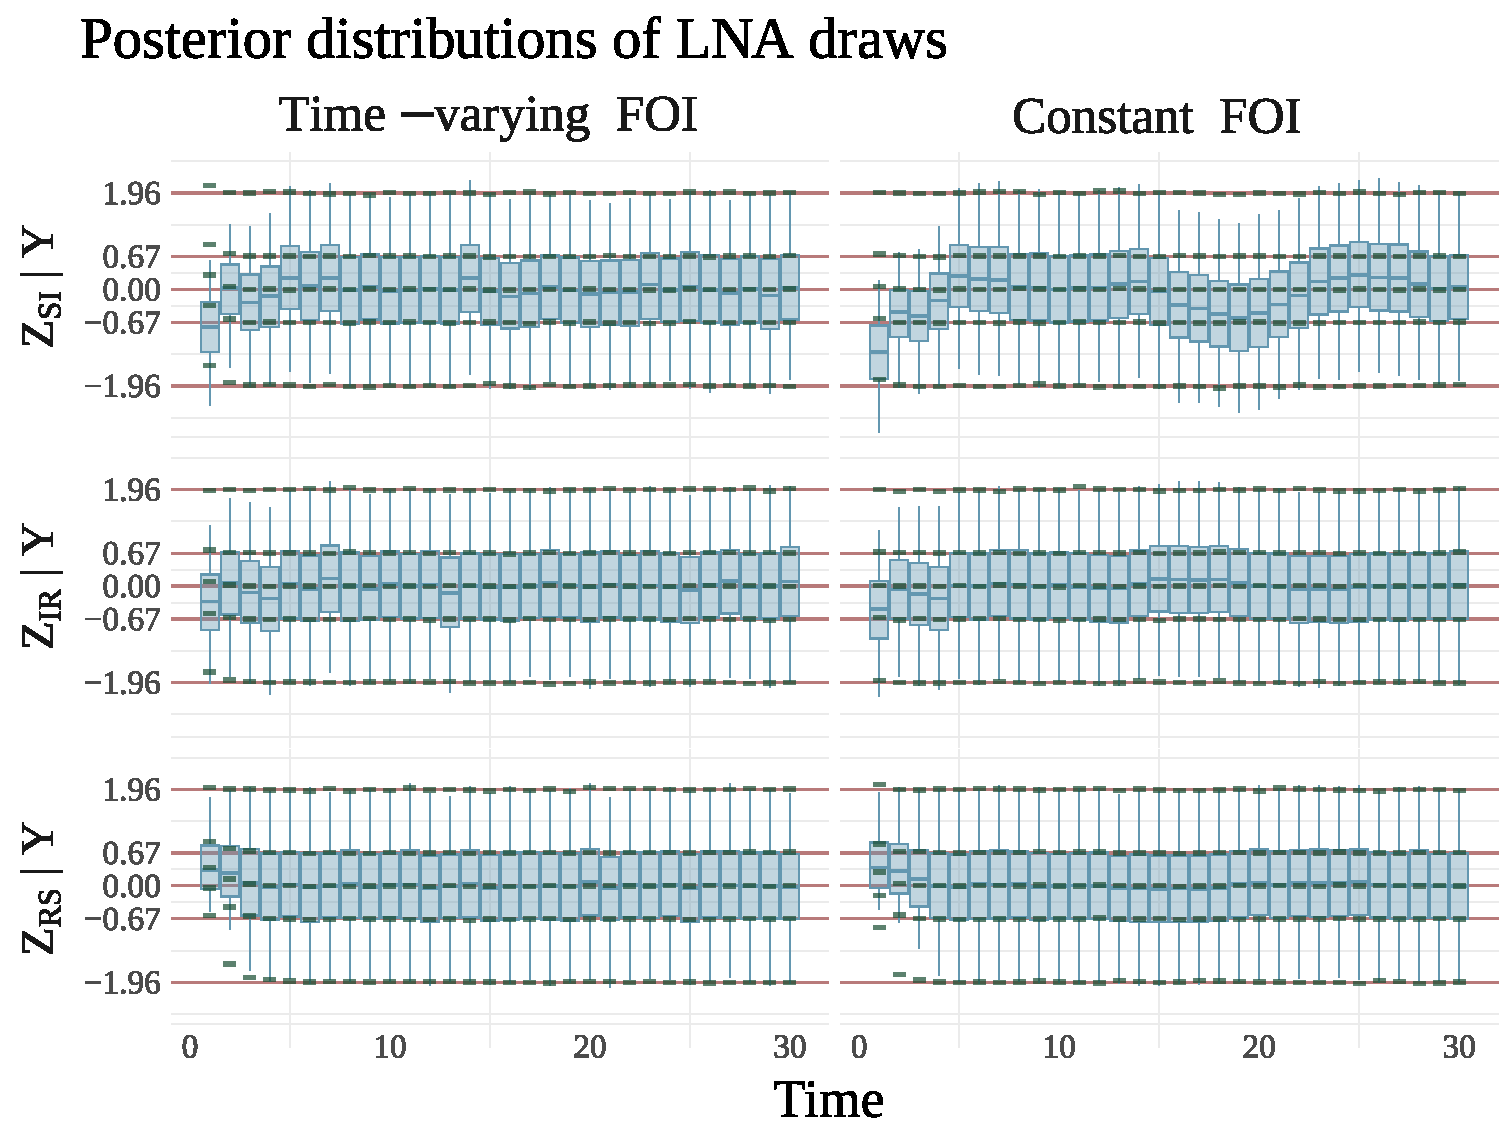
\includegraphics[width=\linewidth]{figures/sinfoi_lna_drawplots}
	\caption[Posterior distributions of LNA draws for SIRS models with time--varying and constant force of infection.]{Posterior distributions of the LNA draws for infection, recovery, and loss of immunity in SIRS models with time--varying and constant force of infection (blue boxplots). The lower and upper whisker tips correspond to the $ 2.5^\mr{th} $ and $ 97.5^\mr{th} $ posterior quantiles, the lower and upper hinges to the $ 25^\mr{th} $ and $ 75^\mr{th} $ quantiles, and the middle hash mark to the posterior median. The solid red lines are the theoretical quantiles of the posterior predictive distribution (or equivalently, the prior distribution) of the LNA draws, drawn at the quantiles of a standard normal distribution corresponding to the boxplot quantiles. The green ticks are the estimated quantiles of the posterior predictive distributions of the LNA draws, accounting for boundary conditions on the state space of the latent process and obtained by simulating LNA paths from the posterior predictive distribution. The posterior distributions of LNA draws are shaded according to the level of posterior shrinkage, computed as one minus the ratio of standard deviations of LNA draws in the posterior and prior.}
	\label{fig:sinfoidrawplots}
\end{figure}
